\documentclass{report}
\usepackage[a4paper]{geometry}
\usepackage{amsmath}
\usepackage{bm}
\usepackage{pgfplots}
\usepackage{ amssymb }
\usepackage{color, soul}
\usepackage[backend=biber]{biblatex}
\addbibresource{references.bib}
\graphicspath{{images/}}


%opening
\title{Directed Study Report\\CSE4DIR}
\author{Ash Hall\\17756156}

\newcommand{\TODO}[1]{\sethlcolor{pink}\hl{\\(#1)\\}}
\newcommand{\FEEDBACK}[1]{\sethlcolor{green}\hl{\\ Feedback: \\#1\\}}
\newcommand{\TOCITE}[2][citation needed]{\textsuperscript{\underline{#1}}}

\begin{document}

	\maketitle
	\thispagestyle{empty}
	\newpage
	\thispagestyle{empty}
	\tableofcontents
	\newpage
	\thispagestyle{empty}
	\newpage
	
	\setcounter{chapter}{1}	
	\chapter*{Directed Study Report}

	\section{Introduction}
	The purpose of this report is to investigate the effects of catastrophic forgetting in artificial neural networks. We will briefly discuss what catastrophic forgetting is and why it occurs, consider some approaches for minimising its effects, then present our experimental findings and discuss the results. \par \par
	As a neural network is improved by optimising the parameters on a per-example basis, they rapidly forget past learned knowledge to ``make way'' for new information. This purportedly occurs due to overlap in internal representations of new and old tasks, where a model may ``re-purpose'' important parameters for a new task, regardless of their importance for old tasks. While catastrophic forgetting is well recognised, its effects are yet to be quantified for comparison. We aim to produce empirical measurements by way of experimentation, and to provide a clear measure of the severity of catastrophic forgetting in artificial neural networks that can be used for comparison moving forward. \par
	
	\section{Transfer Learning}
	The training of a neural network occurs by presenting many examples, and iteratively optimising the weights. A dataset consisting of a small number of examples may be prohibitive to optimisation in this manner, as a model would likely over-fit to the training examples, and not be capable of generalising to novel examples. \emph{Transfer learning} minimising this problem, by allowing a pre-trained model to be re-purposed to a different dataset. \par
	The bulk of an image-classification neural network acts as a \emph{feature-extractor}, with studies\parencite{extractors} showing that a sufficiently-large image dataset leads to a highly-generalisable feature extractor. Transfer learning takes advantage of this property by taking the resultant feature extractor and amending the tail of a neural network to perform classification between different classes. Figure \ref{fig:transferlearning:1} shows a model pre-trained on a large image dataset being adapted to another. \par
	\begin{figure}[h]
		\centering
		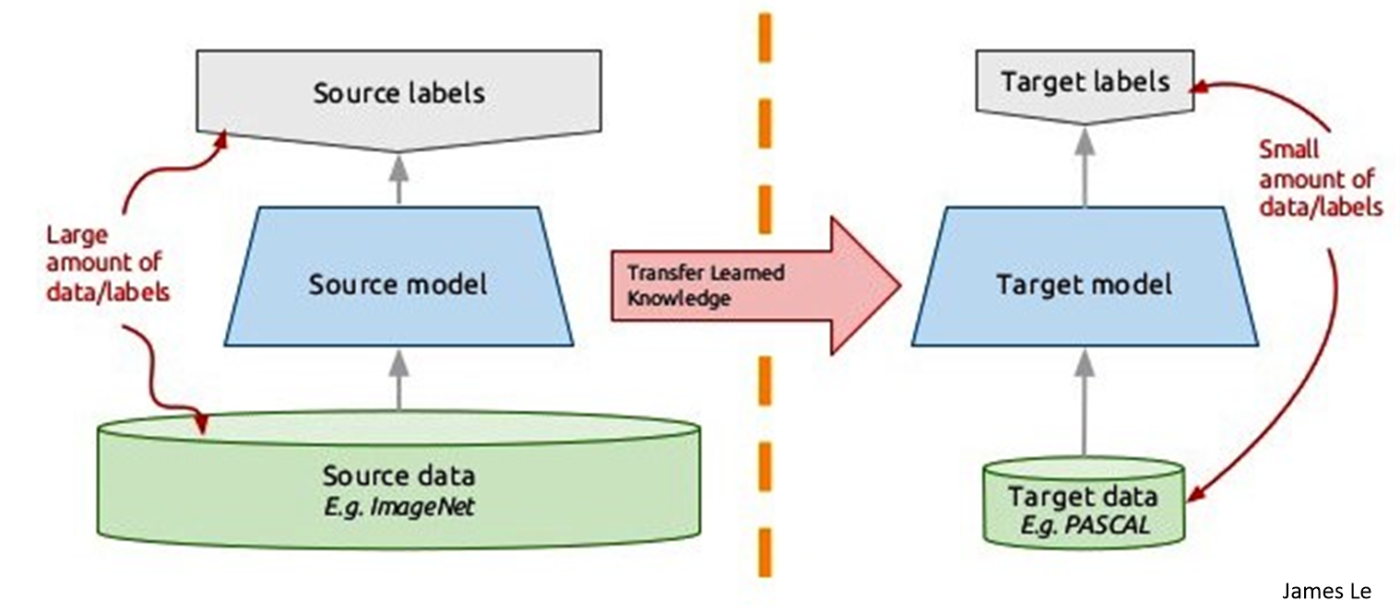
\includegraphics[width=11cm]{transferlearning}
		\caption{Transfer learning overview}
		\label{fig:transferlearning:1}
	\end{figure}
	There are two fundamental problems with this approach. The first is that although this lessens the effects of over-fitting, it doesn't entirely avoid them; training on a very small dataset is still prone to this problem. The other issue is that if you wished to not replace the old dataset classes, but add the new dataset classes to the model, you would need to store examples and repeatedly present them to the network during re-training. This introduces a whole suite of problems including training-example balancing, which we won't address here. \par
	Simply put, while providing strong results, transfer learning is limited in its usability, and is inherently inapplicable to the task of continuous learning -- which we'll address in the following section. \par
	
	\section{Continuous Learning}
	The tendency of neural networks to forget older information is known as catastrophic forgetting; the task of learning from a stream of new information a minimal amount of forgetting is known as continuous learning. \par
	Continuous learning differs from transfer learning in that in order to add classes to an image classifier using transfer learning, examples from the existing classes would need to be \emph{replayed} to the model over time, to ensure that it loses minimal performance on them. A condition of ``true'' continuous learning is that old examples need not be seen again -- this is a reasonable desire, as it would require an increasing amount of training time proportionate to the growing number of images and classes in a dataset. \par

	\subsection{Related Works}
	We will briefly discuss some works related to the task of mitigating catastrophic forgetting -- continuous learning. Although this report is to investigate the effects of catastrophic forgetting and not a survey of related work, it is good to consider other approaches. The following works were built to specifically target catastrophic forgetting, so serve as good points of reference. \par
	
	\subsubsection{Learning to Learn with Backpropagation of Hebbian Plasticity}
	The work by Miconi et. al. \parencite{hebbian} considers an observed biological neurological pattern, where synaptic efficacy (neuron firing strength) increases through persistent stimulation. In this approach, they define a ``Hebbian trace'', which acts as a moving-average of pair-wise synaptic activities. They train a plasticity parameter which determines how much the Hebbian trace affects a pair's connection. \par
	A network gains additional learning capacity by using this technique, as the network learns a sparser internal representation, effectively endowing a larger capacity for knowledge. Although catastrophic forgetting is somewhat reduced, this is not an ideal situation as the models internal capacity remains fixed and as such, is limited to the initial design. \par
	
	\subsubsection{Learning Without Forgetting}
	The technique proposed by Li et. al. \parencite{lwf} seeks to preserve acquired knowledge by recording the existing model's response to new classes examples. They augment the model by adding an additional set of outputs for the new classes, and producing a prediction probability distribution on the old heads using new class examples (figure \ref{fig:lwf:1}). \par
	\begin{figure}[h]
		\centering
		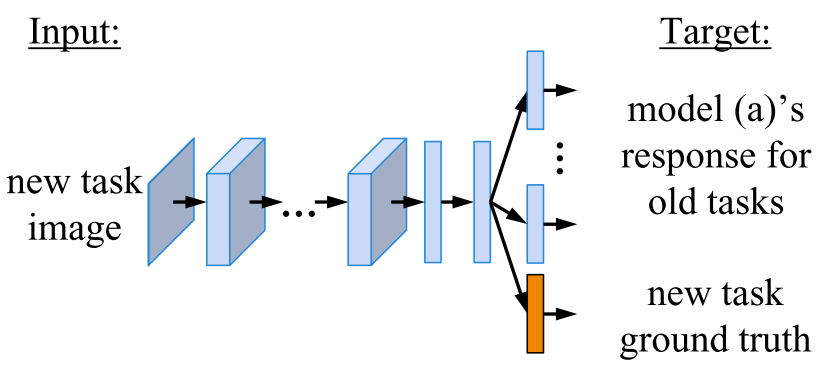
\includegraphics[width=8cm]{lwfarchitecture}
		\caption{Learning Without Forgetting architecture}
		A new output head (orange) is added for each batch of new classes. The model's predicted class probability distribution over the old classes is recorded and incorporated into the loss function. 
		\label{fig:lwf:1}
	\end{figure}
	This is a very literal and largely successful approach to mitigating catastrophic forgetting, but comes with a price -- the user of the model must know prior to performing inference which set of classes the image belongs to. This effectively makes it quite similar to having multiple models, the only difference being that the class groups share a feature extractor. \par

	\subsubsection{Overcoming Catastrophic Forgetting}
	The approach presented by Kirkpatrick et. al. \parencite{lwf} introduces a specialised loss function named \emph{elastic weight consolidation} (EWC), with the sole purpose of preserving old information. They compute a Fischer information matrix -- which is essentially a representation of each weight's importance for the pre-existing classes -- and use it to add an extra term to the loss calculation. With this term included, the loss function has the effect of restraining important parameters to a location in weight-space which provide good performance on the pre-existing classes. \par
	Similarly to \emph{Learning Without Forgetting}, this is an effective technique due to the fact that the retention of knowledge is explicitly embedded in the network's training. \par
	\par
	
	\subsubsection{Summary}
	The aforementioned techniques are designed to minimise the effects of catastrophic forgetting, and each does so in an effective and reasonable manner. That being said, the results yielded by each are incompatible as there is no consistent method for measuring catastrophic forgetting when extending neural networks to more classes. We seek to perform experiments which provide a consistent, coherent basis by which to measure these effects. \par
	

	\section{Environment}
	The following experiments were performed on a computer running the UNIX operating system, with two 8GB Nvidia GTX 1080 graphics cards, a quad-core processor and 64GB of memory. The implementation of the experiments was written using the Python interface for Tensorflow\parencite{tensorflow}, Google's open-source computational framework. Furthermore, Deepmind's Sonnet\parencite{sonnet} was used to provide a simple interface for Tensorflow. The graphing and result logging was done using Tensorboard, a visualisation tool included with Tensorflow. \par
	
	\section{Dataset}
	The experiments described in this report were performed using CIFAR-100\parencite{cifar100}, a dataset consisting of 60,000 32x32 images in 100 classes with 600 images per class. While a small -- in terms of spatial size -- dataset, the 100 classes emulate real-world by having such varied classes as motorcycles, snakes and bottles. \par
	
	\section{Framework}
	The code-base for the experiments is provided in figure \ref{fig:framework:1}, which details a high-level overview of the Python class, module and directory structure. The \texttt{Trainer} trains models, and takes command-line flags to switch the training mode (used when re-training models in different manners). It is also responsible for session management, and writing variables and Tensorboard data to the \texttt{bin} directory. The \texttt{GraphBuilder} abstracts the graph-building operations away from the \texttt{Trainer}, to allow for a cleaner training script. It reads from a configuration \texttt{YAML} file stored in \texttt{configs}, and builds the appropriate \texttt{Model} and \texttt{Optimizer} as required. The data loading, partitioning and sampling is presented via a consistent interface in the \texttt{dataloader} package, with the dataset loaded being specified in the configuration file mentioned. \\
	\begin{figure}[h]
		\centering
		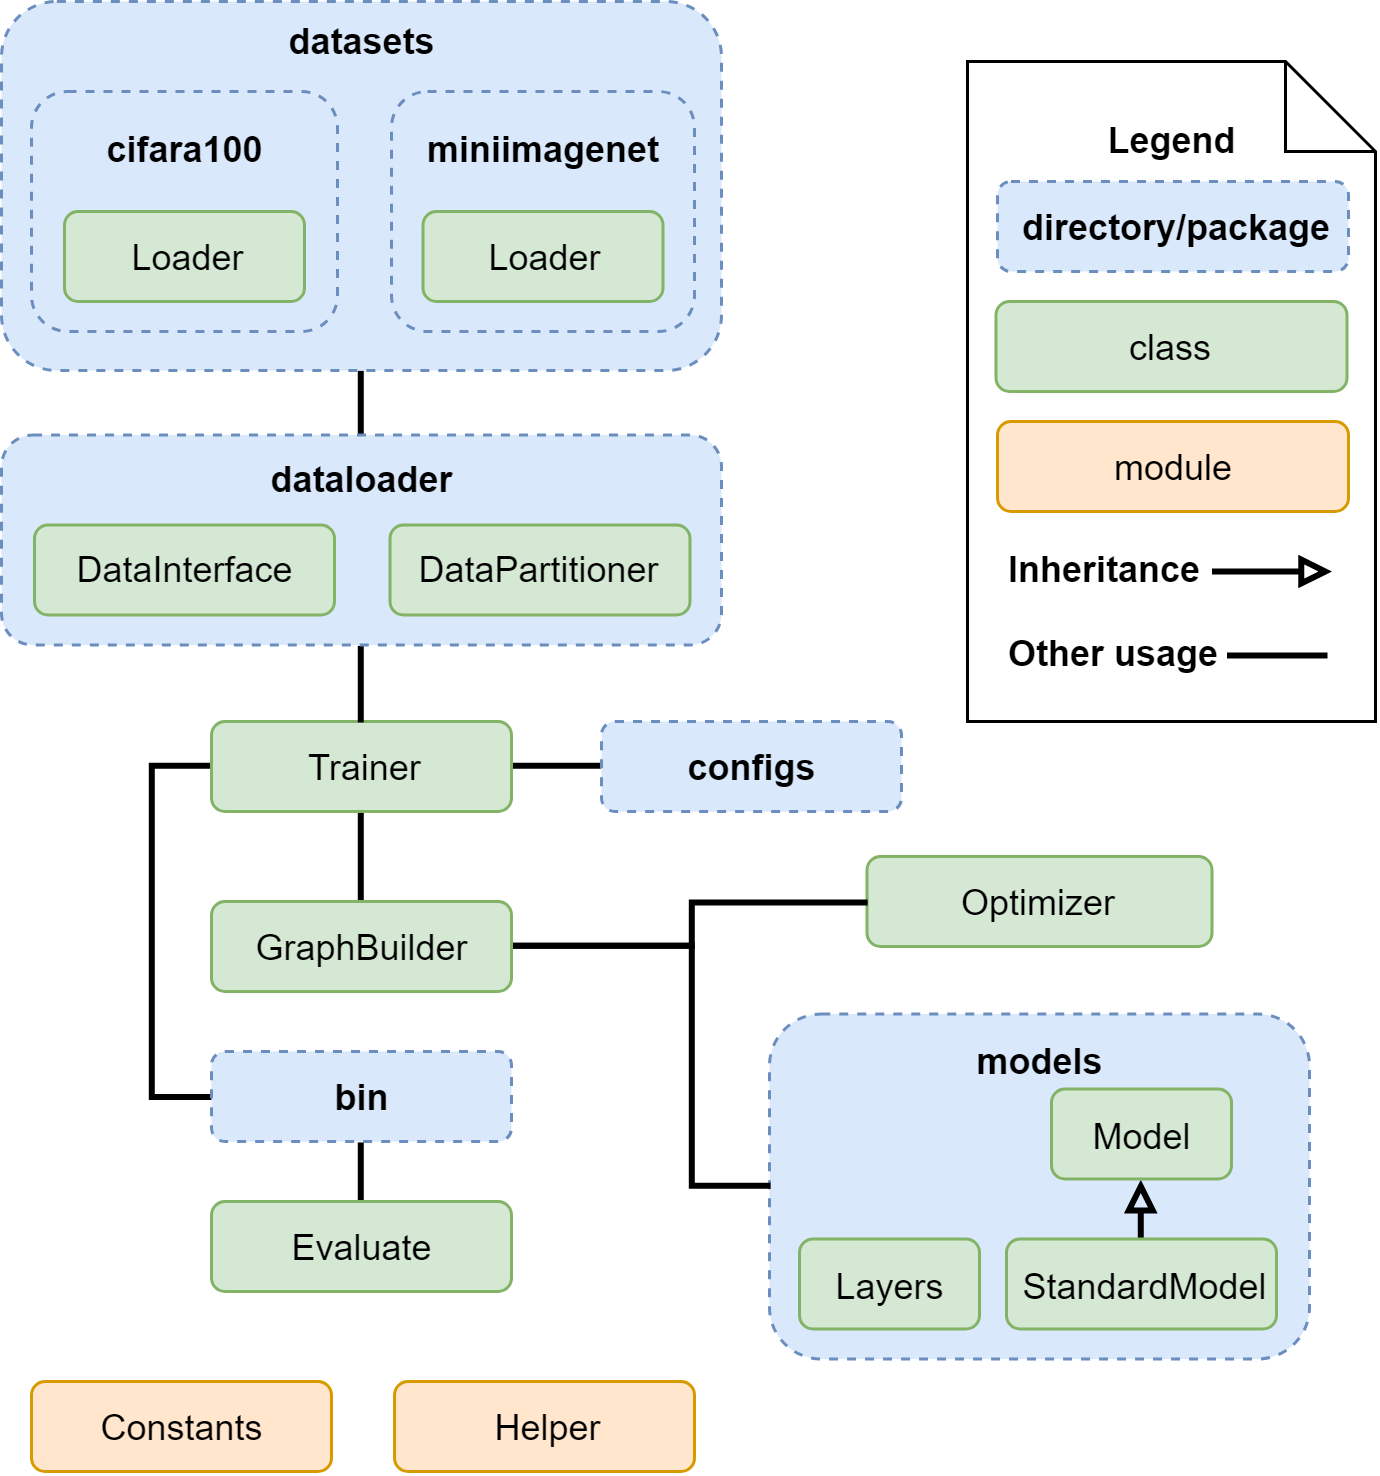
\includegraphics[width=11cm]{codeframework}
		\caption{Code-base Framework}
		A high-level view of the code-base structure. 
		\label{fig:framework:1}
	\end{figure}
	The described modular design provides the ability to quickly perform experiments with different datasets/model configurations. Automatic file-naming in the \texttt{bin} directory allows for experiment results to be easily reviewed and compared in Tensorboard with little effort. \par
	
	\section{Key Terminology}
	\textit{Source classes} refer to a set of classes on which a \textit{source model} has been pre-trained. Similarly, a \textit{target model} is produced by extending a source model's classification ability to also include a set of \textit{target classes} -- a disjoint set of classes to those that the source model was trained on. \par
	
	\section{Pre-Training Procedure}
	Each of the experiments were performed in a two-stage training procedure. The first stage of training was consistent for each experiment, which will now be described. \par
	The models used for training were consistent with other works of the same nature, consisting of four convolutional blocks (figure \ref{fig:convblock:1}) followed a fully-connected output layer. \par
	\begin{figure}[h]
		\centering
		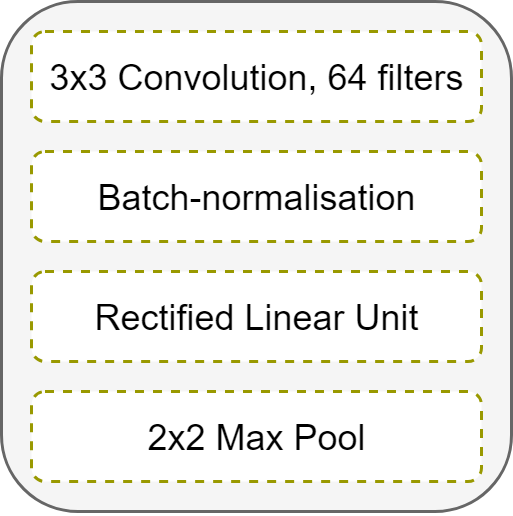
\includegraphics[width=4cm]{convblock}
		\caption{A convolutional block}
		\label{fig:convblock:1}
	\end{figure}
	For CIFAR-100, the number of total classes $N=100$, allowing us the ability to choose a smaller number of \emph{source} and \emph{target} classes and compare results. For a number of per-model source classes $N_S$, we can easily build $N-N_S-1$ overlapping incremental class subsets (figure \ref{fig:subsets:1}).
	For each of these subsets, a model was trained using an Adam optimizer with a learning rate of \TOCITE[?????]{}. Due to the relatively small number of examples in the training/validation sets (500/100), training was stopped after \TOCITE[?????]{} iterations. Stopping at this many training iterations was determined empirically, as training for longer caused the model's performance on the validation set to drop due over-fitting to the training set. \par
	The weights of each model were saved to disk and not modified any further, such that each experiment began with the exact same models. \par
	\begin{figure}[h]
		\centering
		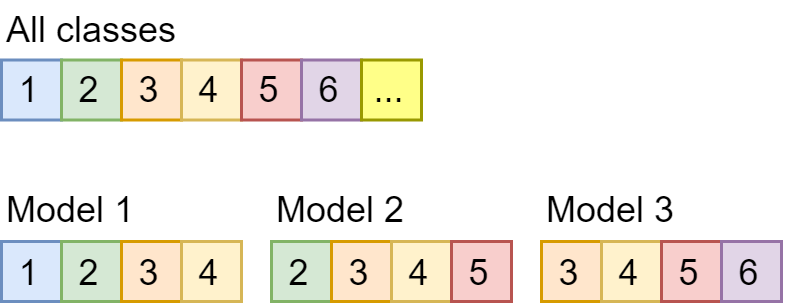
\includegraphics[width=8cm]{modelsubsets}
		\caption{Class subset selection}
		A number of class subsets can easily be selected using an overlapping, incremental selection schema. Example using $N_S = 4$.
		\label{fig:subsets:1}
	\end{figure}

	\section{Metrics}
	A critical aspect is that the metrics reported are truly representative of the amount of catastrophic forgetting occurring. Due to this, each reported value is the average value over $N-N_S-1$ models. \par
	The quality of a model is measured by two components: the accuracy of the target model on the target classes, and the accuracy of the target model on the source classes. The former is a measure of how much the model learns about the target classes; the latter a measure of how much the model retains accuracy on the source classes. Instead of considering the precision in terms of their absolute value, we will instead compute the difference between target model and source model precision. Concretely, for a collection of images, a model will produce a number of correct (C) and incorrect (I) predictions. We can therefore compute the precision for a given model $\bm{\theta}$ on images $\bm{x}$ as in equation \ref{eqn:evaluation:1}.
	\begin{align} \label{eqn:evaluation:1}
	\text{Precision}(\bm{\theta}, \bm{x}) &= \frac{C}{C+I}
	\end{align}
	To compute the relative improvement or deterioration of performance of a model, we simply need to compute the difference in precision between a source model and corresponding target model. It is not possible to measure the source model's performance on the target classes however, as it is in the problem definition that the source model has never seen the target images. In this case, we will consider the source model precision on the source images as a de-facto baseline by which to measure the target model's performance on the target classes. The improvement score equations for source and target classes are shown in equations \ref{eqn:evaluation:2} and \ref{eqn:evaluation:3}, respectively.
	\begin{align} \label{eqn:evaluation:2}
	\text{Score}_S &= \text{Precision}(\bm{\theta}_T, \bm{x}_S) - \text{Precision}(\bm{\theta}_S, \bm{x}_S) \\
	\label{eqn:evaluation:3}
	\text{Score}_T &= \text{Precision}(\bm{\theta}_T, \bm{x}_T) - \text{Precision}(\bm{\theta}_S, \bm{x}_S)
	\end{align}
	By only considering the relative improvement of a model's performance, we don't allow the difficulty of the particular classes to distort our metrics, nor the quality of the source models.
	
	\section{Experiments and Results}
	\TODO{Put a short introduction to the results here after writing them up}
	
	\subsection{Experiment 1}
	\TODO{(These will actually have names, not just experiment 1, 2, ...)}
	\subsection{Experiment 2}
	\TODO{}
	\subsection{Experiment 3}
	TODO{}
		
	\section{Summary}
	\TODO{Summarise the experiment results and what they indicate}
	
	
\end{document}
